%%%%%%%%%%%%%%%%%%%%%%% CHAPTER - 4 %%%%%%%%%%%%%%%%%%%%\\
\chapter{Background and Literature Review}
\label{C4} %%%%%%%%%%%%%%%%%%%%%%%%%%%%
\graphicspath{{Figures/PDF/}{Figures/PNG/}}
\noindent\rule{\linewidth}{2pt}
%%%%%%%%%%%%%%%%%%%%%%%%%%%%%%%%%%%%%%%%%%%%%%%%%%%%%%%%%%%%%%%%%%%%%%%%%%%%%%%%%%%%%%%%%%%%%%%%%%%%%%%%%%%%%%%%%%%%%%%%%%%%%%%%%%%%

%%%%%%%%%%%%%%%%%%%%%%%%%%%%%%%%%%%%%%%%%%%%%%%%%%%%%%%%%%%%%%%%%%%%%%%%%%%%%%%%%%%%%%%%%%%%%%%%%%%%%%%%%%%%%%%%%%%%%%%%%%%%%%%%%%%
% \section{abcs} \label{S2.1}
% Noise is a random variation of brightness in digital images that often occurs due to imperfections in imaging devices and
% ................... \cite{whygaussianity}
% \begin{equation}
% 	v(i)=u(i)+\eta(i) \label{e2.1}
% \end{equation}	
% %%%%%%%%%%%%%%%%%%%%%%%%%%%%%%%%%%%%%%%%%%%%%%%%%%%%%%%%%%%%%%%%%%%%%%%%%%%%%%%%%%%%%%%%%%%%%%%%%%%%%%%%%%%%%%%%%%%%%%%%%%%%%%%%%
% \subsection{xyz} \label{SS2.1}

% \begin{figure}[b!]
% 	\center	
% 	\includegraphics[scale=0.62]{fig2_1} 	
% 	\caption{Image} \label{f2.1}
% \end{figure}
\noindent
The computer systems and the networks of these systems are increasing day by day and security of data share by these networks is being an issue over the years. Security techniques of classical networks cannot be applied here because WSN has certain limitations of resources like energy, memory, CPU, etc. Security mechanism of network must be able to ensure confidentiality, integrity, availability and authenticity.
\section{Intrusion and Intrusion Detection}
An intrusion in any system is an attempt to unauthorized access of system's data or resources. This unauthorized access can be limited to only monitoring and analyzing traffic patterns or it can be an attempt to modify or alter the data packets. Try to make resources busy and unavailable for the intended authorized access is also an intrusion attack. An IDS basically monitors and analyzes the network traffic for any suspicious activity by any of the network node. IDS tries to analyze network behavior and monitors user activity. IDS comes under passive defence category as these system tries to detect intrusion attack rather than preventing attack. These systems can only capable of reporting and alarming to administration to take some action. An IDS which can also take some required action to prevent the attack on its own, is known is Intrusion prevention System (IPS). An IDS is a tool which either installed at network strategic points or at each host to detect any suspicious or malicious behavior. If any such behavior is found which can harm the system nodes or system's activity it notifies to the concerned authority. An IPS can perform all tasks of IDS, in addition to that it can also take desired action on its own to prevent the attack. An ideal IDS tries to minimize false positive rate with high detection rate. Also less energy consumption and faster computation or attack detection is desired feature of IDS. Main components of any IDS are shown in Figure \ref{IDS-Component} \cite{alrajeh2013intrusion} are:
\begin{enumerate}[label=\textbf{\roman*.}]
\item \textbf{Monitoring} This component mainly monitors traffic in the network, availability of resources. Events at each node, network congestion, packet delay, neighbor monitoring is also done by monitoring component.
\item \textbf{Analysis and Detection} This module of IDS implements the detection method for intrusion. It is the main component in the IDS where all monitored traffic patterns, events are analyzed to make decision regarding maliciousness of a node.
\item \textbf{Alarm} Alarm component is responsible for generating responses as alarm to administration if a malicious activity is detected.
\end{enumerate}
\begin{figure}[tp]
\center	
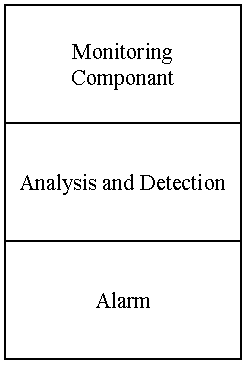
\includegraphics[width=1.75in, height=2.5in] {Figures/PDF/IDS-Components.pdf}
\caption{Components of IDS.}
\label{IDS-Component}	
\end{figure}
\par

% \section{IDS vs IPS}
\noindent
Mainly there are two types of IDS- Rule-based (signature-based) IDS and Anomaly-Based IDS \cite{khan2010framework}. Rule-based IDS can detect previously known attacks with high precision because it takes help of built-in signatures. A rule-based technique was developed \cite{jha2002building} which compares the incoming information with known information. But the problem was that signature-based IDS cannot detect a new attack because its signature is not present. Anomaly-based IDS detects intrusion by monitoring statistical behavioral, can detect the new attack as well as common attacks having more false positive rates i.e. normal packet declared as abnormal. One particular method of threshold was developed to detect the new attacks \cite{xie2011anomaly}. Also, there can be multiple anomaly attacks or some attacks which are consisting of both the attacks, can be detected using Hybrid IDS (HIDS) \cite{sedjelmaci2011novel}. In HIDS, anomaly-based IDS is used as a filter and another one is used as the second level of IDS.
\par
In \cite{mehmood2018secure}, A. Mehmood et al., provided that knowledge-based IDS (KB-IDS) can be applied on cluster-based WSN in order to secure the network. Their method keeps a record of networks internal nodes behavior. They placed knowledge base at the base station and inference engines were used by CHs to access the knowledge base. Because of the continuous monitoring of nodes they were able to sense any potential threat and generate events against them to tackle the attack. This information goes to the BS through the inference engine. The BS concludes and reports back to the CH for the suspicious node.
\par
In \cite{yan2009hybrid}, HIDS on Cluster-based WSN (CWSN) is discussed. CH collects the data from other sensor nodes in that cluster and aggregates it because CH has the higher capability. In this paper it they used 3 models - anomaly detection, misuse detection with decision-making model. First two models were able to detect intrusion from a large number of packets and then results from these two models were combined by decision-making model i.e. if an intrusion has occurred then this model will classify its type. This model then will inform to the administrator about the attack with details.
\par
In \cite{wang2011integrated}, three different individual intrusion detection systems were proposed for the heterogeneous wireless sensor network. An IDS was designed each for the CH, SN and BS. The capability of IDS was depending upon the attack on a particular node. For sink node, IDS has the learning capabilities which helps network to deal with unknown attacks. For CH node, a host-based IDS was proposed without learning capability. This helps the network to detect known attacks and avoid resource wasting, efficiently. To detect and update the class of attack it uses a feedback mechanism. A simple and fast misuse IDS was proposed for SNs.
\par
In \cite{jinhui2018intrusion}, an intrusion detection system is discussed which uses Energy trust in WSN. This method specifically focuses on detecting hybrid DoS attack using effective node energy analysis. This method predicts energy consumption and correlates it with the security of nodes. The method assumes that a sensor node can monitor their own energy level and consumption. It also faces a problem when a node is being under attack by flooding then enemy may try to control the node which can show fake energy information.
\par
In \cite{kalnoor2018detection}, KMP Pattern matching technique was used to detect an intruder. In this, after receiving a pattern, a pattern matching linear time algorithm is used. When features are matched, accordingly a rule is applied to the data packet. Then it calls a plug-in, which is used to find the intrusion. If there is no problem and received packet found to be with the correct pattern then it is forwarded to its neighbors. If a suspicious pattern is detected then it performs three functions namely, alert(): to give warning, logto(): to put information of intrusion in the database table, and trace instruction to trace out the intruder.
\par
In \cite{jianjian2018novel},  IDS based on improved AdaBoost- Radial basis function in Support vector machine is discussed. This system can detect and resist against DoS attack effectively. This system uses RBF-SVM as AdaBoost classifier by training. The IABRBFSVM algorithm is proposed by using the influence of parameter ‘σ’ and model training error ‘e’ on AdaBoost weights. Significantly improves network performance and lifetime, with short computation time and higher detection rate.
\par
In \cite{jin2017multi}, the intrusion detection method is discussed for cluster WSN, which uses trust values and multi-agent framework functioning. Trust value calculation and accuracy are calculated by Mahalanobis distance. Reduction in false positive rate is done by calculating tolerance factor in trust value calculation. This system was scalable as it uses a multi-agent framework. The proposed system was fault tolerant and can detect multiple attacks at the same time with a high detection rate.
\par
In \cite{eik2006intrusion}, anomaly-based IDS was proposed to detect new attacks, initially. Then, in order to understand routing in WSN for intrusion detection, they found a set of features. These features can be applied to all protocols. This IDS was able to detect main attacks in WSN but active sinkhole attacks can be detected effectively. Also, this method consumes less power as it does not require communication between nodes.
\par
In \cite{sedjelmaci2013efficient}, an IDS for cluster-based WSN is discussed. This IDS has different detection frameworks for different levels. The first framework runs at IDS agent at a low level, which is a specification based protocol. The second framework runs at the head node of the cluster (CH, medium level), which is a binary classification protocol. Also, to check trust level of cluster members (agents) a reputation protocol is used by CH. At Base station (higher level) a voting mechanism is applied which is used by CH to monitor its CH neighbors. This system was able to detect blackhole, wormhole, flooding, and selective forwarding attacks. The detection rate was almost 100\%. Time, energy consumed to detect was very low.
\par
In \cite{lu2018intrusion}, an IDS was proposed with an evolving mechanism to extract rules which are used for intrusion detection. Diversity and quantity of rule sets were controlled by measuring the distance between the rules of same class and different class.

\section{IDS - Features and Limitations}
\noindent
Every IDS has certain features like ability to tune to specific attack, helps to meet security regulations, increases efficiency etc and limitations like no prevention of attack, no processing for encrypted data, false positive rate etc. Table \ref{tab:my-table} presents summary of specific features and limitations of research work done in this field. It includes work done in different areas in the field of IDS like Neural Network, Clustering, SVM, Multi-agent trust based schemes.

\begin{longtable}[c]{|p{0.25in}|p{0.75in}|p{1.5in}|p{1.5in}|p{1.5in}|}
\caption{Study of various intrusion detection systems.}
\label{tab:my-table}\\
\hline
\textbf{S.N.} & \textbf{Proposed System} & \textbf{Method} & \textbf{Features} & \textbf{Limitations} \\ \hline
\endfirsthead
%
\multicolumn{5}{c}%
{{\bfseries Table \thetable\ Continued from previous page}} \\
\hline
\textbf{S.N.} & \textbf{Proposed System} & \textbf{Method} & \textbf{Features} & \textbf{Limitations} \\ \hline
\endhead
%
1. & A. Mehmood et al. \cite{mehmood2018secure} & Cluster-based IDS, uses knowledge base for storing patterns, inference engine. & SN monitors traffic and send observed events to CH which is further forwarded to BS where action against malicious node is taken. & Heavy load on SN inside the cluster, faster battery drainage for CH. \\ \hline
2. & S. S. Wang et al. \cite{wang2011integrated} & 3 different IDS for heterogeneous WSN- For sink node, IDS has the learning capabilities, For CH node, a Host based IDS, misuse IDS for SNs. & Can detect known, unknown attacks, avoids resource wasting, uses feedback mechanism. & Consumes high energy as it uses learning and feedback mechanism. \\ \hline
3. & D. Jianjian et al. \cite{jianjian2018novel} & Improved AdaBoost-Radial basis function in Support Vector Machine. & Detects DoS attack efficiently, improves network performance, short computation, high detection rate. & Only Focused on DoS attack, can;t detect multiple attacks. \\ \hline
4. & X. Jin et al. \cite{jin2017multi} & Uses trust values and multi-agent framework functioning, uses Mahalanobis distance. & Reduction in false positive rate, scalable system, fault tolerant, can detect multiple attacks at the same time. & Trust value calculation and accuracy are calculated by Mahalanobis distance. \\ \hline
5. & H. Sedjelmaci et al. \cite{sedjelmaci2013efficient} & 3 different detection frameworks- specification based, binary classification protocol, vote mechanism. & Detection rate was almost 100\%. Time, energy consumed to detect was very low. & System was able to detect only black hole, wormhole, flooding and selective forwarding attacks. \\ \hline
6. & A. Saeed et al. \cite{saeed2016random} & Uses Random Neural Network, without any dedicated hardware. & Very effective in low-power WSN, detects any performance degradation anomaly attack, can also detect previously unknown attacks. & Computation time, energy consumption was high as compared to others at the cost of accuracy. \\ \hline
7. & W. Meng et al. \cite{meng2014efm} & K-nearest neighbor (KNN) algorithm with filtering. Built with three components. & Resolves issues of network packet overload, false alarm rate. Provides efficient signature matching. & Expensive in terms of time for computation. \\ \hline
8. & G. Gowrisona et al. \cite{gowrison2013minimal} & Uses Neural Network with KDD Cup99 data. & An adaptive method with higher detection accuracy. Detects DoS attacks with enhanced rules by learning. Efficient computational complexity of O(n). & No knowledge management system, implementation has to be in cloud-based environment. \\ \hline
\end{longtable}

\section{Classification of IDS}
IDS classification has two broad categories - Signature-based and Anomaly-based, which are based on intrusion detection strategy. IDS can also be classified based on the location of data in two categories - Host-based and Network-based. More classification categories are shown in Figure \ref{IDS-Classification} \cite{alrajeh2013intrusion, farooqi2009intrusion} are described below.

\begin{figure}[ht]
\center	
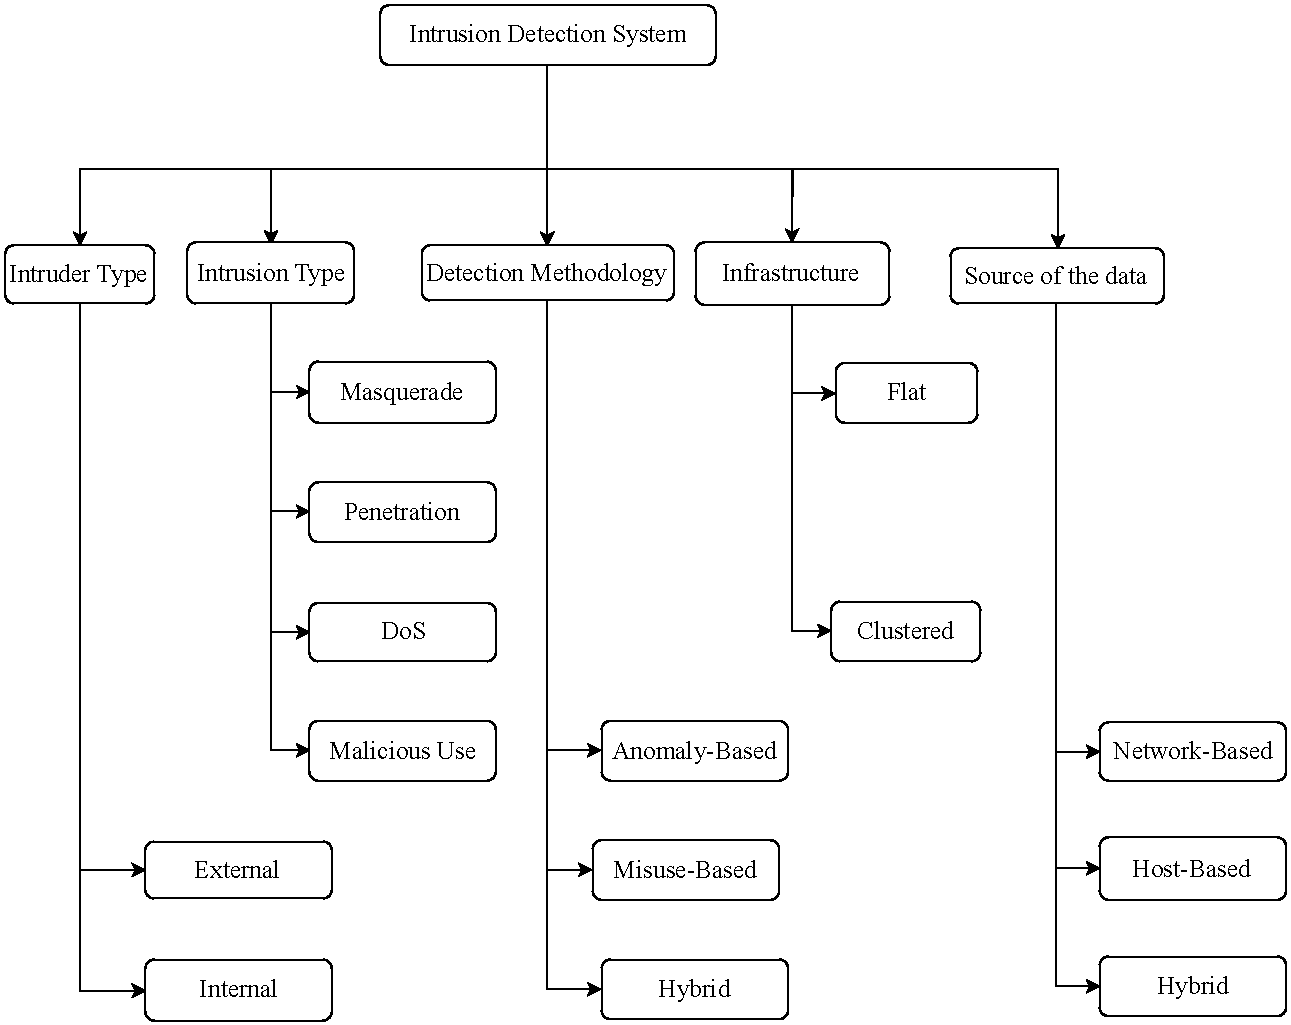
\includegraphics[width=\textwidth, height=5in] {Figures/PDF/IDS_Classification.pdf}
\caption{Classification of IDS.}
\label{IDS-Classification}	
\end{figure}

\subsection{Detection Method}
IDS functionality is defined by the detection method. It describes how a detection system will behave in order to detect any malicious activity in the network. Research field in WSN mainly focuses on these following detection methods.
\begin{itemize}
  \item{\textbf{Anomaly-based} Anomaly-based IDS uses heuristic approaches to classify network activities as malicious or normal. This detection method finds the deviation from normal behavior and uses threshold value to classify attacks. To flag operation as an anomaly, the regular observation of system must be there to accommodate system changes. This may lead to performance overhead. It sometimes fail to detect well-known attack but works well in case of unknown attacks. In [4] an IDS is proposed which is capable of learning and detecting new attacks using unsupervised neural network. Anomaly-based identification can be factual based, information based or AI based.}
  \item{\textbf{Misuse-based (Signature or Rule-based)} In this detection method predefined rules are already there against attacks to tackle them. Using this method one can detect previously known attack with high detection rate by comparing the new attack signature with known signatures and predefined rules. If there is a new attack, signature-based detection would not be able to compare with any reference signature (profile) hence this attack won’t be detected. In \cite{ioannis2007towards, krontiris2007intrusion}, a signature based IDS is presented. Every node has IDS so it is host based IDS. The architecture design for \cite{ioannis2007towards} is such that it detects data-packet drop and false routing attack and \cite{krontiris2007intrusion} is designed to detect only sinkhole attack.}
  \item{\textbf{Hybrid IDS} These systems uses the combination of anomaly-based and misuse-based detection to detect new attacks using learning algorithms and  to detect well-known attacks, respectively. Hybrid systems are increasingly productive regarding detection rate with low false positive rate. Also, these system uses high computation and hence results in more energy consumption. A hybrid IDS is proposed in \cite{li2008intruder} which uses distributive algorithm to train support vector machine (SVM) and create misuse detection model.}
\end{itemize}
\subsection{Source of Data}
IDS can be classified in 3 categories based upon the location of the data. It describes the location of the data where it is monitored. Data can be monitored on individual nodes or on the strategic point of network.
\begin{itemize}
    \item{\textbf{Network-Based} NIDS are deployed at strategic points so that it can monitor the packets transmission in network that is coming and going out to all network devices. This monitoring of data is then analyzed and compared with the signatures of known attacks. It is easy to deploy on the network boundary  with low cost where it can monitor all traffic.}
    \item{\textbf{Host-Based} HIDS is implemented on individual host systems in the network and monitors all incoming and outgoing traffic instead of the whole network. HIDS is more helpful if the malicious node is inside the network.}
    \item{\textbf{Hybrid IDS} It uses mobile agents to efficiently use a combination of NIDS and HIDS. Performance of hybrid IDS of better in terms of detection rate compared to NIDS and HIDS but hybrid system consumes more energy in detection process.}
\end{itemize}
\subsection{Intruder Type}
IDS classification based on  an intruder node can be of two types - internal and external. It describe the location of the compromised node. In external intruder, attacker or compromised node is not present in the network whereas in case of internal intruder, it is present in the network. Internal intruder further can be classified as selfish node and malicious node in the way in which they affect the network's operation. Selfish node uses the network to forward own data packets, saves battery life for own operations, no cooperation in data forwarding, no direct damage to other nodes. On the other hand, malicious node damages other nodes, not focused on saving own battery life, tries to damage network services.
\subsection{Intrusion Type}
It describes a way of attack in which system is compromised. In masquerade attack, attacker uses fake identity to gain unauthorized access. Penetration is an attempt to unauthorized access by breaching networks security. In DoS attack, attacker node tries to extra use of network resource so authenticated users can’t access resources. Malicious use of resources is an attack on network resource.

\subsection{Infrastructure Type}
IDS can be classified into 2 groups based on network infrastructure - Flat and Clustered. In flat infrastructure, all nodes can participate in all networking activities because it is assumed that all the nodes in the network have equal capabilities. In clustered, nodes are grouped which is known as clusters and each group is assigned a head known as CH.

\section{Summary}
This chapter discusses about big threat to sensor netwaork i.e. intrusion and its detection. Various detection techniques involving neural networks, fuzzy logic, trust values have been discussed. Features and limitations of certain detection mechanism have also been enlisted in tabuler form. Major limitations in detection for current systems is that there is always a trade-off between accuracy and real-time performance. One detection method cannot detect all the intrusions because of new attacks are being introduced as time is progressing. Also, resource usage limitations makes is more difficult. To design an ideal IDS, which is capable of detecting all attacks with high accuracy and with limites resource use, will always be an challenge in this domain of research.